\documentclass[11pt]{article}

\usepackage{fullpage}
\usepackage{amsmath, amssymb, bm, cite, epsfig, psfrag}
\usepackage{graphicx}
\usepackage{float}
\usepackage{amsthm}
\usepackage{amsfonts}
\usepackage{listings}
\usepackage{cite}
\usepackage{hyperref}
\usepackage{tikz}
\usepackage{enumerate}
\usepackage{listings}
\usepackage{mathtools}
\lstloadlanguages{Python}
\usetikzlibrary{shapes,arrows,positioning,trees}

\DeclareFixedFont{\ttb}{T1}{txtt}{bx}{n}{9} % for bold
\DeclareFixedFont{\ttm}{T1}{txtt}{m}{n}{9}  % for normal
% Defining colors
\usepackage{color}
\definecolor{deepblue}{rgb}{0,0,0.5}
\definecolor{deepred}{rgb}{0.6,0,0}
\definecolor{deepgreen}{rgb}{0,0.5,0}
\definecolor{backcolour}{rgb}{0.95,0.95,0.92}

\def\del{\partial}
\def\ds{\displaystyle}
\def\ts{\textstyle}
\def\beq{\begin{equation}}
\def\eeq{\end{equation}}
\def\beqa{\begin{eqnarray}}
\def\eeqa{\end{eqnarray}}
\def\beqan{\begin{eqnarray*}}
\def\eeqan{\end{eqnarray*}}
\def\nn{\nonumber}
\def\binomial{\mathop{\mathrm{binomial}}}
\def\half{{\ts\frac{1}{2}}}
\def\Half{{\frac{1}{2}}}
\def\N{{\mathbb{N}}}
\def\Z{{\mathbb{Z}}}
\def\Q{{\mathbb{Q}}}
\def\R{{\mathbb{R}}}
\def\C{{\mathbb{C}}}
\def\argmin{\mathop{\mathrm{arg\,min}}}
\def\argmax{\mathop{\mathrm{arg\,max}}}
\def\diag{\mathop{\mathrm{diag}}}
\def\x{\times}
\def\limn{\lim_{n \rightarrow \infty}}
\def\liminfn{\liminf_{n \rightarrow \infty}}
\def\limsupn{\limsup_{n \rightarrow \infty}}
\def\GV{Guo and Verd{\'u}}
\def\MID{\,|\,}
\def\MIDD{\,;\,}

\newtheorem{proposition}{Proposition}
\newtheorem{definition}{Definition}
\newtheorem{theorem}{Theorem}
\newtheorem{lemma}{Lemma}
\newtheorem{corollary}{Corollary}
\newtheorem{assumption}{Assumption}
\newtheorem{claim}{Claim}
\def\qed{\mbox{} \hfill $\Box$}
\setlength{\unitlength}{1mm}

\def\bhat{\widehat{b}}
\def\ehat{\widehat{e}}
\def\phat{\widehat{p}}
\def\qhat{\widehat{q}}
\def\rhat{\widehat{r}}
\def\shat{\widehat{s}}
\def\uhat{\widehat{u}}
\def\ubar{\overline{u}}
\def\vhat{\widehat{v}}
\def\xhat{\widehat{x}}
\def\xbar{\overline{x}}
\def\zhat{\widehat{z}}
\def\zbar{\overline{z}}
\def\la{\leftarrow}
\def\ra{\rightarrow}
\def\MSE{\mbox{\small \sffamily MSE}}
\def\SNR{\mbox{\small \sffamily SNR}}
\def\SINR{\mbox{\small \sffamily SINR}}
\def\arr{\rightarrow}
\def\Exp{\mathbb{E}}
\def\var{\mbox{var}}
\def\Tr{\mbox{Tr}}
\def\tm1{t\! - \! 1}
\def\tp1{t\! + \! 1}
\def\Tm1{T\! - \! 1}
\def\Tp1{T\! + \! 1}


\def\Xset{{\cal X}}

\newcommand{\one}{\mathbf{1}}
\newcommand{\abf}{\mathbf{a}}
\newcommand{\bbf}{\mathbf{b}}
\newcommand{\dbf}{\mathbf{d}}
\newcommand{\ebf}{\mathbf{e}}
\newcommand{\gbf}{\mathbf{g}}
\newcommand{\hbf}{\mathbf{h}}
\newcommand{\pbf}{\mathbf{p}}
\newcommand{\pbfhat}{\widehat{\mathbf{p}}}
\newcommand{\qbf}{\mathbf{q}}
\newcommand{\qbfhat}{\widehat{\mathbf{q}}}
\newcommand{\rbf}{\mathbf{r}}
\newcommand{\rbfhat}{\widehat{\mathbf{r}}}
\newcommand{\sbf}{\mathbf{s}}
\newcommand{\sbfhat}{\widehat{\mathbf{s}}}
\newcommand{\ubf}{\mathbf{u}}
\newcommand{\ubfhat}{\widehat{\mathbf{u}}}
\newcommand{\utildebf}{\tilde{\mathbf{u}}}
\newcommand{\vbf}{\mathbf{v}}
\newcommand{\vbfhat}{\widehat{\mathbf{v}}}
\newcommand{\wbf}{\mathbf{w}}
\newcommand{\wbfhat}{\widehat{\mathbf{w}}}
\newcommand{\xbf}{\mathbf{x}}
\newcommand{\xbfhat}{\widehat{\mathbf{x}}}
\newcommand{\xbfbar}{\overline{\mathbf{x}}}
\newcommand{\ybf}{\mathbf{y}}
\newcommand{\zbf}{\mathbf{z}}
\newcommand{\zbfbar}{\overline{\mathbf{z}}}
\newcommand{\zbfhat}{\widehat{\mathbf{z}}}
\newcommand{\Ahat}{\widehat{A}}
\newcommand{\Abf}{\mathbf{A}}
\newcommand{\Bbf}{\mathbf{B}}
\newcommand{\Cbf}{\mathbf{C}}
\newcommand{\Bbfhat}{\widehat{\mathbf{B}}}
\newcommand{\Dbf}{\mathbf{D}}
\newcommand{\Gbf}{\mathbf{G}}
\newcommand{\Hbf}{\mathbf{H}}
\newcommand{\Ibf}{\mathbf{I}}
\newcommand{\Kbf}{\mathbf{K}}
\newcommand{\Pbf}{\mathbf{P}}
\newcommand{\Phat}{\widehat{P}}
\newcommand{\Qbf}{\mathbf{Q}}
\newcommand{\Rbf}{\mathbf{R}}
\newcommand{\Rhat}{\widehat{R}}
\newcommand{\Sbf}{\mathbf{S}}
\newcommand{\Ubf}{\mathbf{U}}
\newcommand{\Vbf}{\mathbf{V}}
\newcommand{\Wbf}{\mathbf{W}}
\newcommand{\Xhat}{\widehat{X}}
\newcommand{\Xbf}{\mathbf{X}}
\newcommand{\Ybf}{\mathbf{Y}}
\newcommand{\Zbf}{\mathbf{Z}}
\newcommand{\Zhat}{\widehat{Z}}
\newcommand{\Zbfhat}{\widehat{\mathbf{Z}}}
\def\alphabf{{\boldsymbol \alpha}}
\def\betabf{{\boldsymbol \beta}}
\def\betabfhat{{\widehat{\bm{\beta}}}}
\def\epsilonbf{{\boldsymbol \epsilon}}
\def\mubf{{\boldsymbol \mu}}
\def\lambdabf{{\boldsymbol \lambda}}
\def\etabf{{\boldsymbol \eta}}
\def\xibf{{\boldsymbol \xi}}
\def\taubf{{\boldsymbol \tau}}
\def\sigmahat{{\widehat{\sigma}}}
\def\thetabf{{\bm{\theta}}}
\def\thetabfhat{{\widehat{\bm{\theta}}}}
\def\thetahat{{\widehat{\theta}}}
\def\mubar{\overline{\mu}}
\def\muavg{\mu}
\def\sigbf{\bm{\sigma}}
\def\etal{\emph{et al.}}
\def\Ggothic{\mathfrak{G}}
\def\Pset{{\mathcal P}}
\newcommand{\bigCond}[2]{\bigl({#1} \!\bigm\vert\! {#2} \bigr)}
\newcommand{\BigCond}[2]{\Bigl({#1} \!\Bigm\vert\! {#2} \Bigr)}
\newcommand{\tran}{^{\text{\sf T}}}
\newcommand{\herm}{^{\text{\sf H}}}
\newcommand{\bkt}[1]{{\langle #1 \rangle}}
\def\Norm{{\mathcal N}}
\newcommand{\vmult}{.}
\newcommand{\vdiv}{./}


% Python style for highlighting
\newcommand\pythonstyle{\lstset{
language=Python,
backgroundcolor=\color{backcolour},
commentstyle=\color{deepgreen},
basicstyle=\ttm,
otherkeywords={self},             % Add keywords here
keywordstyle=\ttb\color{deepblue},
emph={MyClass,__init__},          % Custom highlighting
emphstyle=\ttb\color{deepred},    % Custom highlighting style
stringstyle=\color{deepgreen},
%frame=tb,                         % Any extra options here
showstringspaces=false            %
}}

% Python environment
\lstnewenvironment{python}[1][]
{
\pythonstyle
\lstset{#1}
}
{}

% Python for external files
\newcommand\pythonexternal[2][]{{
\pythonstyle
\lstinputlisting[#1]{#2}}}

% Python for inline
\newcommand\pycode[1]{{\pythonstyle\lstinline!#1!}}

\begin{document}

\title{Homework 11: Decision Tree and Random Forest\\Solutions}
\author{Prof. Yao Wang}
\date{}

\maketitle

\section*{Problem 1}

Figure~\ref{fig:p1} shows a partition of the feature space with two features each in the range of 0 to 1. Draw a decision tree that can realize this partition.

\begin{figure}[h]
\centering
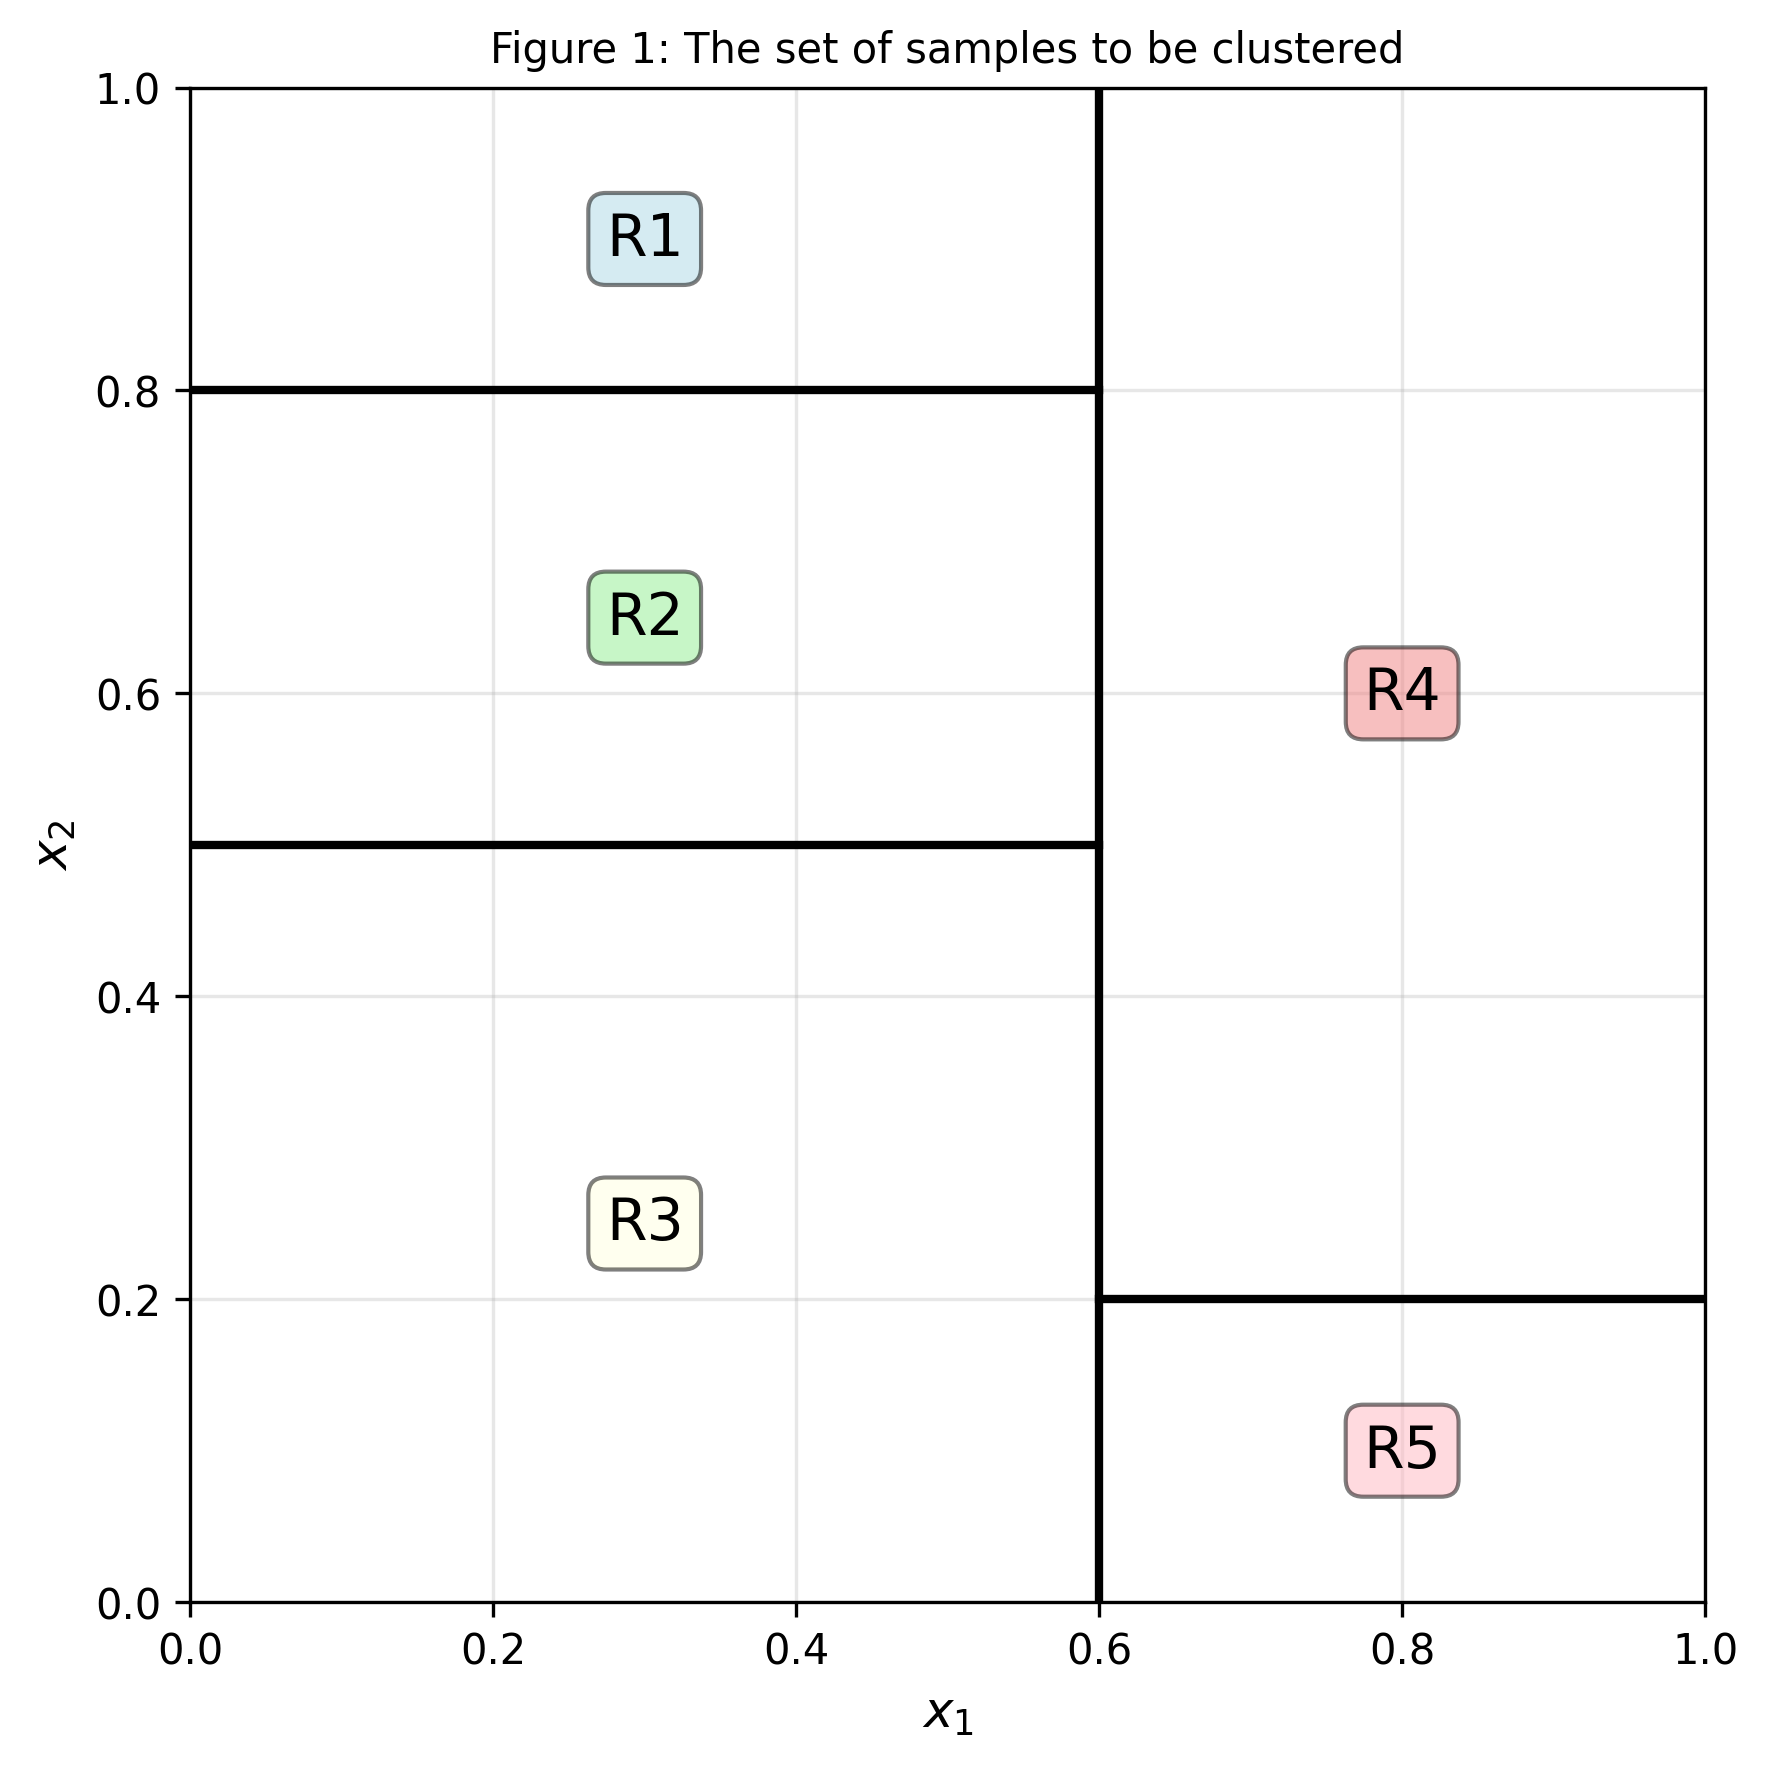
\includegraphics[width=0.3\columnwidth]{p1_partition.png}
\caption{Partition of the feature space} \label{fig:p1}
\end{figure}

\subsection*{Solution}

Analyzing Figure~\ref{fig:p1}, the partition consists of 5 regions (R1 through R5) created by axis-aligned splits:
\begin{itemize}
\item Vertical split at $x_1 = 0.6$
\item Horizontal splits at $x_2 = 0.8$, $x_2 = 0.5$ (for $x_1 \leq 0.6$), and $x_2 = 0.2$ (for $x_1 > 0.6$)
\end{itemize}

The decision tree that realizes this partition is:

\begin{figure}[h]
\centering
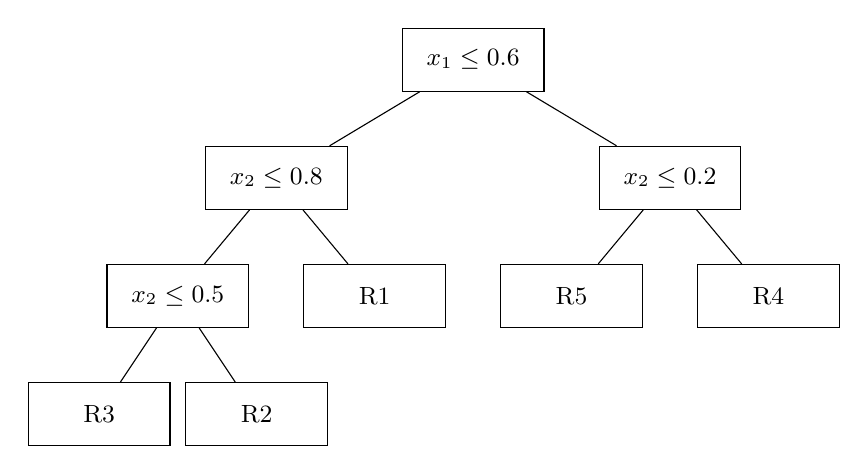
\begin{tikzpicture}[
  level 1/.style={sibling distance=5cm},
  level 2/.style={sibling distance=2.5cm},
  level 3/.style={sibling distance=2cm},
  every node/.style={rectangle, draw, align=center, minimum width=1.8cm, minimum height=0.8cm, font=\small}
]
\node {$x_1 \leq 0.6$}
  child {node {$x_2 \leq 0.8$}
    child {node {$x_2 \leq 0.5$}
      child {node {R3}}
      child {node {R2}}
    }
    child {node {R1}}
  }
  child {node {$x_2 \leq 0.2$}
    child {node {R5}}
    child {node {R4}}
  };
\end{tikzpicture}
\caption{Decision tree for Problem 1} \label{fig:tree1}
\end{figure}

\textbf{Explanation:}
\begin{enumerate}
\item \textbf{Root node}: Split on $x_1 \leq 0.6$ to separate left and right halves of the feature space.
\item \textbf{Left branch} ($x_1 \leq 0.6$): 
  \begin{itemize}
  \item Split on $x_2 \leq 0.8$ to separate top region from middle/bottom regions
  \item If $x_2 > 0.8$: Region R1
  \item If $x_2 \leq 0.8$: Further split on $x_2 \leq 0.5$
    \begin{itemize}
    \item If $x_2 \leq 0.5$: Region R3
    \item If $x_2 > 0.5$: Region R2
    \end{itemize}
  \end{itemize}
\item \textbf{Right branch} ($x_1 > 0.6$):
  \begin{itemize}
  \item Split on $x_2 \leq 0.2$ to separate bottom and top regions
  \item If $x_2 \leq 0.2$: Region R5
  \item If $x_2 > 0.2$: Region R4
  \end{itemize}
\end{enumerate}

This tree structure correctly partitions the feature space into the 5 regions shown in Figure~\ref{fig:p1}.

\newpage

\section*{Problem 2}

Figure~\ref{fig:p2} shows a set of training samples for a binary classification problem. Design a decision tree using the misclassification rate as the loss function.  Note that given this simple problem, you should be able to ``eyeball'' the correct partition threshold for each possible splitting variable,  instead of using exhaustive search. That is, for each split, consider both features ($x_1$ and $x_2$), but for each feature you should be able to eyeball the proper splitting threshold.

\begin{figure}[h]
\centering
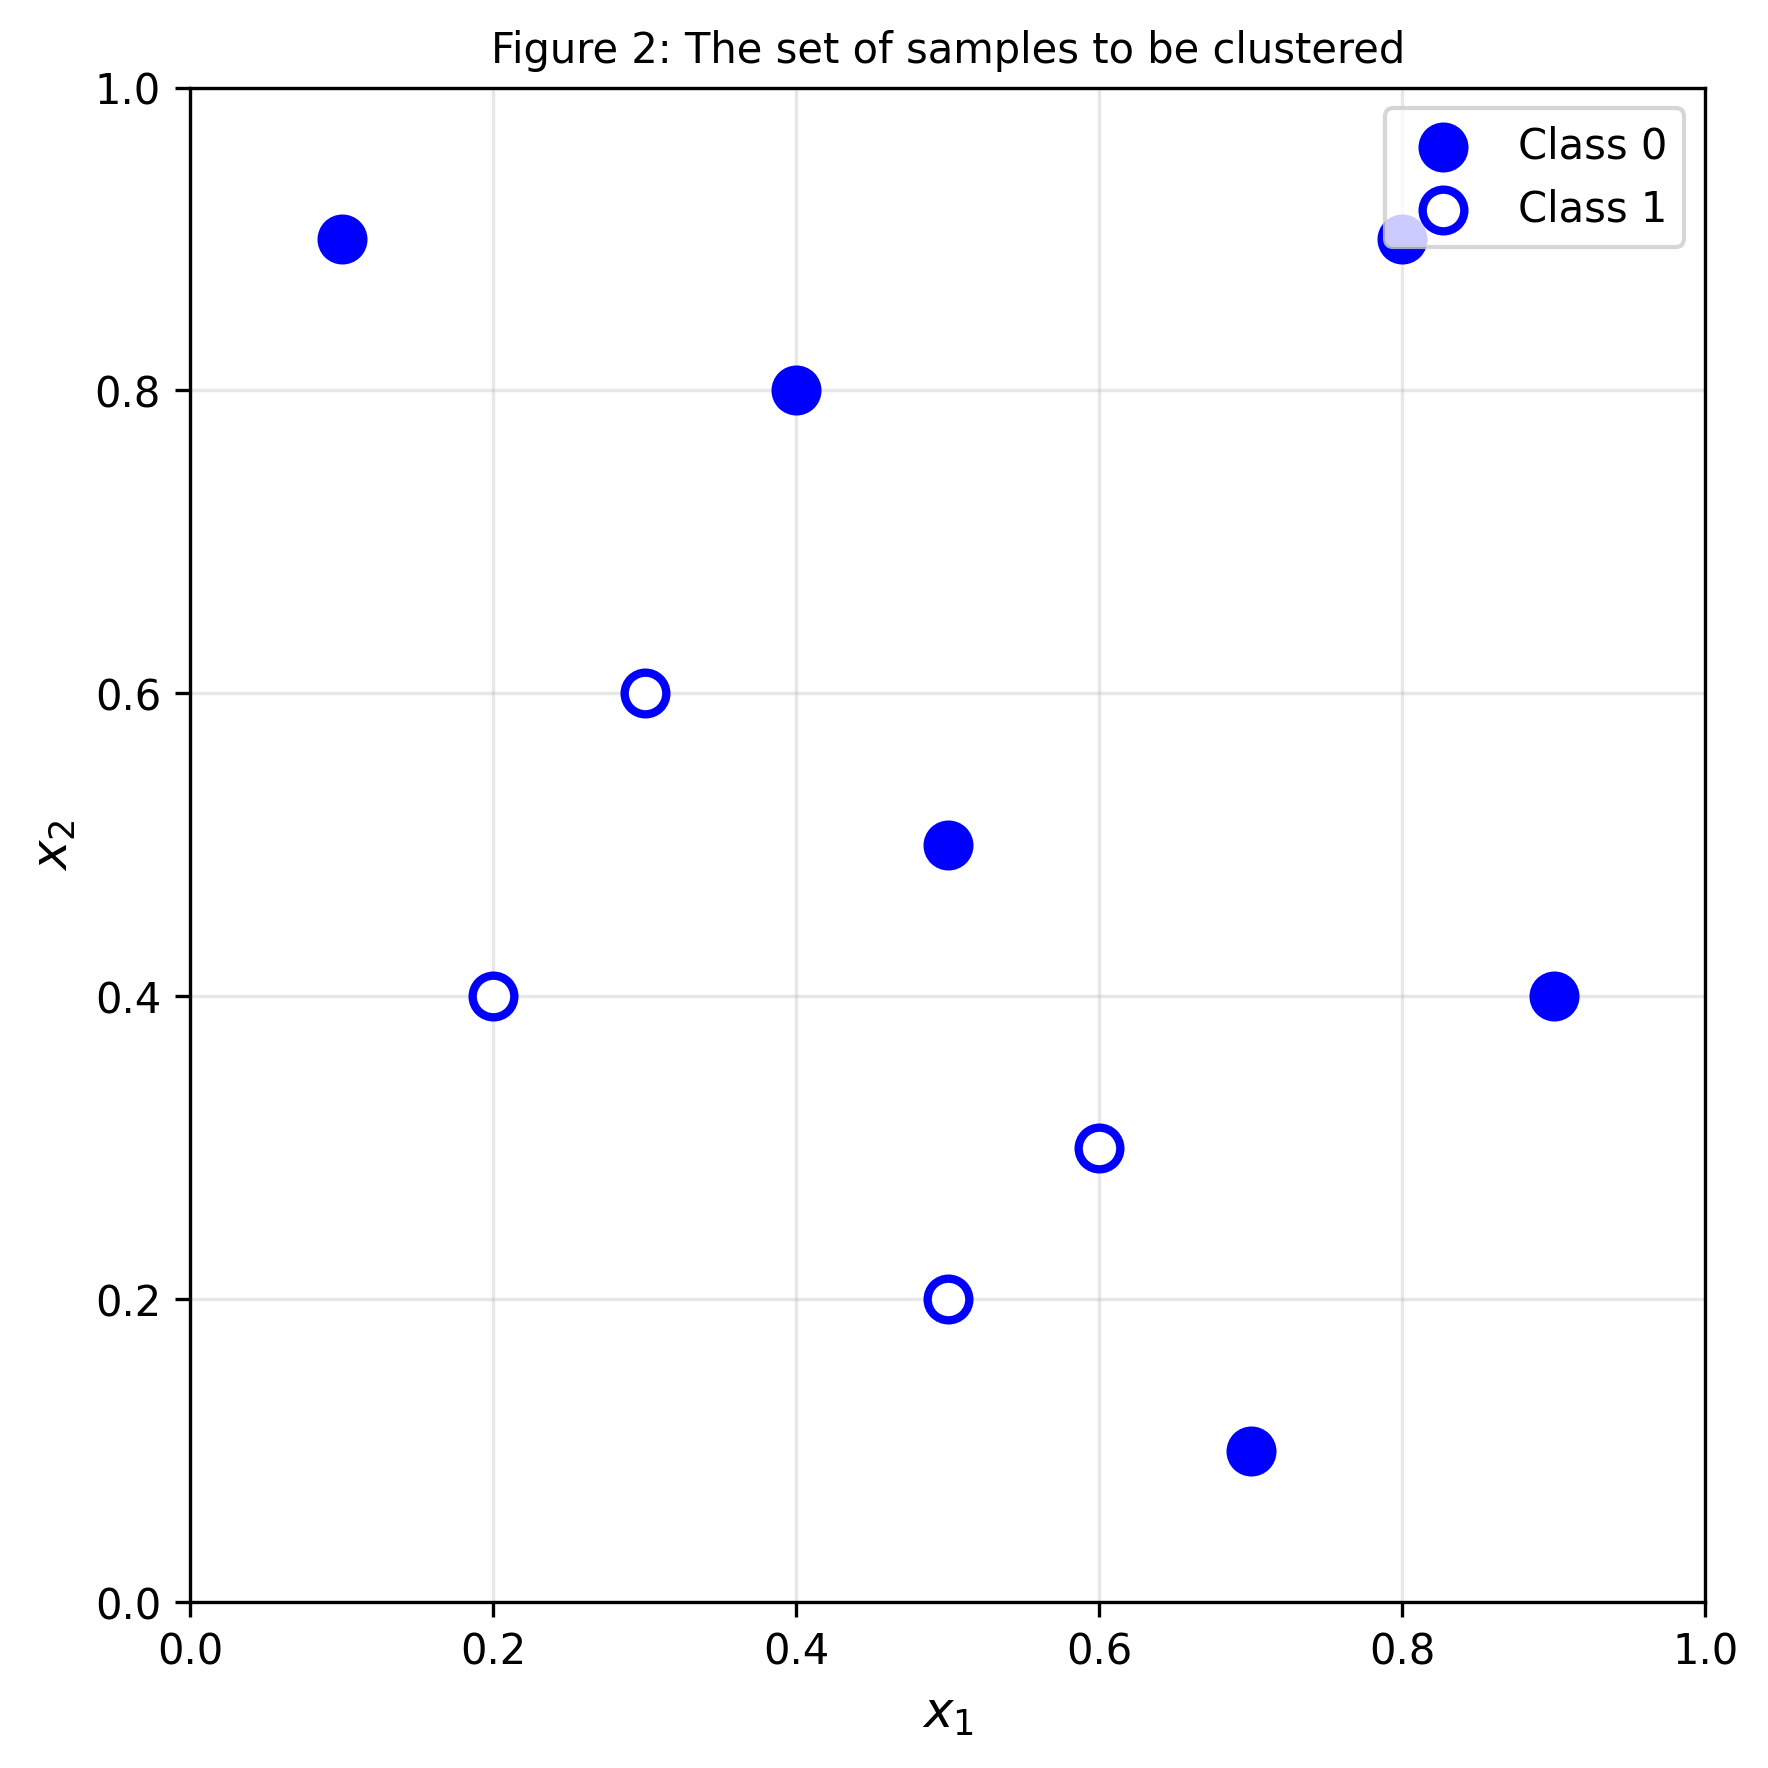
\includegraphics[width=0.3\columnwidth]{p2_classification.png}
\caption{Training samples for binary classification} \label{fig:p2}
\end{figure}

\subsection*{Solution}

From Figure~\ref{fig:p2}, we have:
\begin{itemize}
\item \textbf{Class 0} (filled circles): 6 points at approximately (0.1, 0.9), (0.4, 0.8), (0.8, 0.9), (0.9, 0.4), (0.7, 0.1), (0.5, 0.5)
\item \textbf{Class 1} (empty circles): 4 points at approximately (0.2, 0.4), (0.3, 0.6), (0.6, 0.3), (0.5, 0.2)
\item \textbf{Total}: 10 samples
\end{itemize}

\textbf{Step 1: Root Node Split}

We evaluate splits on both $x_1$ and $x_2$ to minimize misclassification rate. The misclassification rate is:
\[
\text{Misclassification Rate} = \frac{\text{Number of misclassified samples}}{\text{Total number of samples}}
\]

\textbf{Option 1: Split on $x_2 \leq 0.5$}
\begin{itemize}
\item \textbf{Left child} ($x_2 \leq 0.5$): Class 0: 2 points; Class 1: 3 points
  \begin{itemize}
  \item Majority: Class 1, misclassify 2 Class 0 points
  \end{itemize}
\item \textbf{Right child} ($x_2 > 0.5$): Class 0: 4 points; Class 1: 1 point
  \begin{itemize}
  \item Majority: Class 0, misclassify 1 Class 1 point
  \end{itemize}
\item \textbf{Total misclassification}: 3/10 = 0.3
\end{itemize}

\textbf{Option 2: Split on $x_1 \leq 0.5$}
\begin{itemize}
\item \textbf{Left child} ($x_1 \leq 0.5$): Class 0: 2 points; Class 1: 2 points
  \begin{itemize}
  \item Tie (assign Class 0), misclassify 2 Class 1 points
  \end{itemize}
\item \textbf{Right child} ($x_1 > 0.5$): Class 0: 4 points; Class 1: 2 points
  \begin{itemize}
  \item Majority: Class 0, misclassify 2 Class 1 points
  \end{itemize}
\item \textbf{Total misclassification}: 4/10 = 0.4
\end{itemize}

\textbf{Best split}: $x_2 \leq 0.5$ with misclassification rate 0.3

\textbf{Step 2: Split Right Child ($x_2 > 0.5$)}

This node has 4 Class 0 and 1 Class 1. We can further split to reduce misclassification.

\textbf{Option: Split on $x_1 \leq 0.5$}
\begin{itemize}
\item \textbf{Left child} ($x_1 \leq 0.5$): Class 0: 2 points; Class 1: 1 point
  \begin{itemize}
  \item Majority: Class 0, misclassify 1 Class 1 point
  \end{itemize}
\item \textbf{Right child} ($x_1 > 0.5$): Class 0: 2 points; Class 1: 0 points
  \begin{itemize}
  \item Pure Class 0, misclassify 0
  \end{itemize}
\item \textbf{Total misclassification}: 1/5 = 0.2 (improvement from 1/5 = 0.2)
\end{itemize}

\textbf{Step 3: Split Left Child of Root ($x_2 \leq 0.5$)}

This node has 2 Class 0 and 3 Class 1. We can further split.

\textbf{Option: Split on $x_1 \leq 0.4$}
\begin{itemize}
\item \textbf{Left child} ($x_1 \leq 0.4$): Class 0: 0 points; Class 1: 1 point
  \begin{itemize}
  \item Pure Class 1, misclassify 0
  \end{itemize}
\item \textbf{Right child} ($x_1 > 0.4$): Class 0: 2 points; Class 1: 2 points
  \begin{itemize}
  \item Tie (assign Class 0), misclassify 2 Class 1 points
  \end{itemize}
\item \textbf{Total misclassification}: 2/5 = 0.4
\end{itemize}

The final decision tree is:

\begin{figure}[h]
\centering
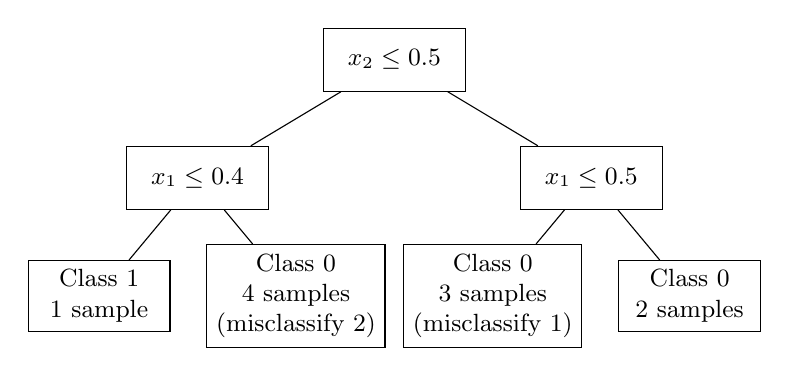
\begin{tikzpicture}[
  level 1/.style={sibling distance=5cm},
  level 2/.style={sibling distance=2.5cm},
  level 3/.style={sibling distance=2cm},
  every node/.style={rectangle, draw, align=center, minimum width=1.8cm, minimum height=0.8cm, font=\small}
]
\node {$x_2 \leq 0.5$}
  child {node {$x_1 \leq 0.4$}
    child {node {Class 1\\1 sample}}
    child {node {Class 0\\4 samples\\(misclassify 2)}}
  }
  child {node {$x_1 \leq 0.5$}
    child {node {Class 0\\3 samples\\(misclassify 1)}}
    child {node {Class 0\\2 samples}}
  };
\end{tikzpicture}
\caption{Decision tree for Problem 2} \label{fig:tree2}
\end{figure}

\textbf{Final Misclassification Rate:}
\begin{itemize}
\item Root left branch: 2 misclassified out of 5 samples
\item Root right branch: 1 misclassified out of 5 samples
\item \textbf{Total: 3/10 = 0.3 (30\% misclassification rate)}
\end{itemize}

This tree minimizes the misclassification rate for the given training data.

\end{document}
